\documentclass{llncs}
\usepackage{makeidx}  % allows for indexgeneration
\usepackage[utf8]{inputenc}
\usepackage{amsmath}
\usepackage{graphicx} \graphicspath{ {../img/} }


\begin{document}
\pagestyle{headings}  % switches on printing of running heads
\addtocmark{The difference operation between templates of binary cellular automata} % additional mark in the TOC

\title{The difference operation between templates of binary cellular automata}

\titlerunning{Difference operation between templates}

\author{Zorandir Soares\inst{2} \and Maurício Verardo\inst{2} \and
Pedro Paulo Balbi de Oliveira\inst{1}\inst{2}}

\authorrunning{Zorandir Soares, Maurício Verardo, and Pedro de Oliveira} 

\tocauthor{Zorandir Soares, Maurício Verardo, and Pedro de Oliveira}

\institute{Universidade Presbiteriana Mackenzie\\
Faculdade de Computação e Informática
\and
Pós-Graduação em Engenharia Elétrica e Computação\\
Rua da Consolação 896, Consolação\\
01302-907 São Paulo, SP - Brazil\\
\email{zorandir@gmail.com}\\
\email{mauricio.verardo@gmail.com}\\
\email{pedrob@mackenzie.br}}

\maketitle              % typeset the title of the contribution

\begin{abstract}
A cellular automata template consist in a notation that has recently been introduced to represent families of cellular automata that share a given property. This paper introduces the operation of difference between templates, used to find cellular automata that have a given property but lack another one. This paper also introduce a process called \textit{exception templates} that is required to this operation. Experimental results of both techniques are illustrated with examples in the space of elementary cellular automata.
\keywords{cellular automata, rule space, templates, difference between templates, exception templates.}
\end{abstract}
%
\section{Introduction}
\label{sec:introducao}
Cellular automata (CAs) are dynamical systems typically discrete in time, space and states.
CAs can produce behavior of great complexity based on simple rules of local action \cite{wolfram2002}. The study of classical problems of cellular automata, like the parity problem \cite{Betel2013} and the density classification problem \cite{deOliveira2014density} can help to understand how this complex behavior emerges.

The most basic approach to find a suitable solution to classic problems consists in testing each of the rules of a particular family of CAs in order to see if any of these rules are able to solve the problem. However, this approach shows to be inefficient or impractical for larger families of CAs, which is the most usual panorama in literature.

Evolutionary computing is constantly used to deal with larger families. This type of algorithm has proven very effective to find solutions for the density classification problem \cite{wolz2008very}.

Another strategy to find suitable rules is restricting the search space by rules that have a given property. To represent a subspace with a particular property without the need of enumerate all of the space rules, one can use \textit{templates}, as proposed in \cite{deOliveira2014,deOliveira2014b}.

There are two operations that can be applied to templates: \textit{expansion} and \textit{intersection} \cite{deOliveira2014,deOliveira2014b}. In this paper we introduce a new operation, named \textit{difference between templates} and the operation that generates the \textit{exception templates}. Moreover, application of these operations are presented in this paper with practical examples.
% Atualmente, não temos "a lot of operations", só temos a expansão e a interseção. Pode dizer isso e citar os artigos onde elas estão explicadas. Tente sempre evitar termos meio vagos como "a lot of" e etc.
% Po, "difference between templates" é um nome meio grande...hahaha será que não tem outro melhor?

This paper is organized in sections. The next section, \ref{sec:automatos_celulares}, presents some basic concepts about cellular automata. Following, Section \ref{sec:templates} presents more details about templates and its major operations. The Section \ref{sec:diferenca_entre_templates_e_templates_de_excecao} introduces the operation of difference between templates and the operation that generates what we call the \textit{exception templates}, as well as their applications. Finally, the Section \ref{sec:consideracoes_finais} makes closing remarks about the news algorithm.

\section{Cellular Automata}
\label{sec:automatos_celulares}
Cellular Automata are simple mathematical idealizations of natural systems \cite{wolfram1994cellular}. They consist of a lattice of discrete cells, each of which can be on one of a finite set of states in a given time step. The values (or states) of the cells evolve in discrete time steps usually according to deterministic rules that specify the state of each cell according to the states of their neighboring cells \cite{wolfram1994cellular}.% "Cellular Automata are simple mathematical idealizations of natural systems" está identico ao autor. "which can be on one of a"?

Conventionally, it is assumed that a cellular automaton cells have $k$ states which are represented by integer values in the range of $[0, k-1]$ The state of a cell is changed by the local function of the automaton (a rule), formed by the state transitions set of a cell, based on its current state and in the states of adjacent cells. To update the values of a cell by local functions, usually a radius $r$ is defined as the number of adjacent cells to be analyzed in each direction by local functions.

A family (space) of cellular automata, is defined by the radius $r$ and the number of states $k$. One-dimensional cellular automata with $r=1$ e $k=2$ are called the family of elementary cellular automata.

To refer to the rules of a space, it is common to use the number obtained by the outputs decimal representation of the state transitions, sorting the lexicographically neighborhoods from largest to smallest state; for instance, in the elementary space, the number of the rules corresponds to the decimal sequence formed by the 8-bit output, arranged from the neighborhood 111 to 000.

The number of rules in a space is provided by $k^{k^{2r+1}}$, making it easy to realize that any increase in the values of $k$ and $r$ generates families with a large amount of rules. An approach to handle this problem is to use static properties as a hint on how the CA will behave during its evolution. A static property is obtained directly from the CA's rule table. The use of static properties can highly restrict the initial search space. With templates can be represented a set of rules with certain static property.

In order to explain how templates work, it is important to understand the properties of number conservation, internal symmetry and color blindness, that will be used in later examples.

\subsection{Number Conservation}
Number conservation is a static property that determines that the sum of the states of a particular cellular automata should not change during the CA's evolution, regardless of the initial configuration.

According to Boccara and Fukś \cite{boccara2002}, a CA is conservative when each of its local function $f$, applied in every neighborhood $(\alpha_0,\alpha_1, \dots, \alpha_{n-1})$ satisfies the conditions described in Eq. \ref{eq:conservativeCA}.
\begin{equation}
\begin{split}
f(\alpha_0,\alpha_1, \dots,\alpha_{n-1}) = \alpha_0 + (\sum_{i=0}^{n-2}f(0_0,0_1, \dots,0_i,\alpha_1,\alpha_2, \dots,\alpha_{n-1}) \\- f(0_0,0_1, \dots,0_i,\alpha_0,\alpha_1, \dots,\alpha_{n-i-1}))
\label{eq:conservativeCA}
\end{split}
\end{equation}

\subsection{Internal symmetry}
To grasp the internal symmetry property, the comprehension of the concept of dynamic equivalence of rules is needed. The following explanations are valid for binary rules, although it is possible to generalize to $k$ states.

Given a transitions table of an CA, there are three changes that can be applied and results in a dynamically equivalent behavior to CAs: \textit{reflection}, \textit{combination} and \textit{composition}. Reflection is the transformation obtained reflecting the bits of the neighborhoods transitions table. The conjugation is obtained by reversing all the states of the cells of the transitions table. Finally, the composition is obtained making reflection and conjugation, regardless of the order.

  \begin{figure}[!ht]
    \centering
    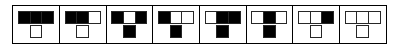
\includegraphics[width=0.7\textwidth]{fig_ruleIcon60.png}
    \caption{Transitions table of the rule 60 of the elementary space.}
    \label{fig:table60}
  \end{figure}
  \begin{figure}[!ht]
    \centering
    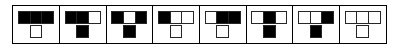
\includegraphics[width=0.7\textwidth]{fig_ruleIcon102.png}
    \caption{Transitions table of the rule 102 from the elementary space, obtained through transformation by reflection applied to the transitions table of rule 60.}
    \label{fig:table102}
  \end{figure}

To illustrate these dynamic equivalence as well the transformations, consider the transition table of Rule 60 of the elementary space, as shown in Figure \ref{fig:table60}. When applying the transformation by reflection in rule 60 we obtain the Rule 102 of the elementary space, illustrated in Figure \ref{fig:table102}.

The internal symmetry is defined by the number of state transitions which remain identical after applied a specific transformation. For example, the rule 60 from the elementary CAs has a value of internal symmetry by reflection equal to 4, because it shares the state transitions $((1,1,1),0)$, $((1,0,1),1)$, $((0,1,0),1)$ e $ ((0,0,0),0)$ with the resulting rule of its transformation by reflection, the rule 102.

\subsection{Color blind cellular automata}
A CA is considered color blind when it is invariant to the application of permutations in the states of transition table \cite{salo2013color}. Naturally, there is generally $k!$ permutations, but only one in the binary case, which can be described as $\{0 \to 1 ,\, 1 \to 0\}$. 

The property color blind is directly related to transformation by conjugation, and the color blind rules have maximum internal symmetry by conjugation.

\section{Templates}
\label{sec:templates}
Template is a generalization of the state transition tables of CAs through variables. A template can represents a rule set, which in turn can presents particular property. The templates were created and implemented by De Oliveira and Verardo \cite{deOliveira2014} and are currently available at the library \textit{open source CATemplates} \cite{CATemplates} on GitHub.

Formally, a \textit{template} is an $n$-tuple formed by $k^{2r+1}$ items, wherein each item $i$ represents a function $g_i(x_{k^{2r+1}-1},x_{k^{2r+1}-2},\dots,x_1,x_0)$. The variables $x_i$ can assume any state between 0 and $k-1$. Can be limited the possible values of $x_i$ by the notation $x_i \in C$, in which $C$ is a set representing the possible values of $x_i$. %TODO verificar essa função $g_i$

As an example, the template of the elementary space $T_1 = (1,1,1,1,1-x_1,x_2,x_1,0)$ represents all the rules which have at position 0 (always from right to left) state 0, at positions 4, 5, 6 and 7 the state 1, at positions 1 and 2 any state in the interval $ [0, k-1] $ and in position 3 the complementary state to the value of position 1. Therefore the template $T_1$ represents the set of elementary cellular automata in its decimal form $\{248,242,252,246\}$ or in binary form as presented below:
\begin{displaymath}
\{(1,1,1,1,1,0,0,0),(1,1,1,1,0,0,1,0),(1,1,1,1,1,1,0,0),(1,1,1,1,0,1,1,0)\}
\end{displaymath}

The process of finding all the rules represented by a template is called \textit{expansion}. There are implemented in the library \textit{CATemplates} \cite{CATemplates} several generators algorithms of templates representing rules with certain property. %TODO Inverter frase
 The template $T_{comp} = (1 - x_0, 1 - x_4, 1 - x_2, x_4, 1 - x_1, x_2, x_1, x_0)$ of the elementary CAs, for example, when expanded generates only rules that have a maximum internal symmetry by composition. But the template $T_{inv} = (1 - x_0, 1 - x_1, 1 - x_2, 1 - x_3, x_3, x_2, x_1, x_0)$ of the elementary CAs expands only the rules with color blind property.

Besides the possibility of expansion of templates, it has been developed by De Oliveira e Verardo \cite{deOliveira2014b} an algorithm to generate templates that represent the intersection between two sub-spaces of rules represented by templates. To illustrate, consider the search for a rule set that are both color blind and have maximum internal symmetry by composition. To find this rule set is necessary to perform two steps: first one must match the two templates that represent the desired properties, thus forming an equation system; then to solve the equations, relationships are generated between the variables that, when applied to templates received as input will result in the template representing the intersection.

As an example, consider the template $T_{comp}$ representing rules with a maximum symmetry by composition and the template $T_{inv}$representing color blind rules, both with $k=2$ and $r=1$. The first step to finding the intersection between these two template is equate them generating the equation system represented by Eq. \ref{eq:interseccaoP1}:
\begin{equation}
\left\{\begin{matrix}
1 - x_0 & = & 1 - x_0 \\
1 - x_4 & = & 1 - x_1 \\
1 - x_2 & = & 1 - x_2 \\
x_4   & = & 1 - x_3 \\
1 - x_1 & = & x_3   \\
x_2   & = & x_2   \\
x_1   & = & x_1   \\
x_0   & = & x_0   \\
\end{matrix}\right.
\label{eq:interseccaoP1}
\end{equation}

Then, the system is solved yielding the solution set $S = \{x_3 = 1-x1, x_4 = x_1\}$. This solution set is then applied as a set of replacements to the templates received as parameter. If the templates received as parameter does not show variables constraints, the result of both replacements can be chosen, ending the process and resulting in the template $(1 - x_0, 1 - x_1, 1 - x_2, x_1, 1 - x_1, x_2, x_1, x_0)$, which is the intersection of templates $T_{comp}$ and $T_{inv}$and, therefore, all the rules of the elementary space which at the same time is color blind and present maximum symmetry by composition.

If at least one of the templates presents variables with restriction, a second step should be carried out. Therefore, the expressions that restrict the variables are extracted, generating a set which is then translated into a new equation system to be solved, whose solution set is then applied as a set of replacements in the templates passed as parameter.

Inspired by the intersection operation, we introduce in this article the operation of difference between templates.

\section{Difference Between Templates and Exception Templates}
\label{sec:diferenca_entre_templates_e_templates_de_excecao}

The difference operation has two templates as an input parameter, which we will call $T_{minuend}$ and $T_{subtrahend}$. This operation output will result in a set of templates that represents all the rules represented by the template $T_{minuend}$ and are not represented by the $T_{subtrahend}$.

The difference operation is a process with several steps. The first consists in a process of intersection between the two selected templates set as parameters, resulting in a template $T_i$. If there is no intersection between the two original template, the result of the difference is the actual $T_{minuend}$. If there intersection, the intersection of template $T_i$ is matched to the template $T_{minuend}$, thereby generating logical combinations of equations. Then the algorithm removes the tautological equations and applies a negation operation in the equation, which in the binary case is to just make the permutations $\rho = (0 \to 1, 1 \to 0)$ to the result of the equations. Then, the logical operator is exchanged from $\wedge$ to $\vee$ and the system generated by this process is solved, thereby generating a set of replacement sets that should be applied to the template $T_{minuend}$. If the replacement set is empty or invalid (ie, reference non existing rules in the space, as exemplified below), all the rules pertaining to $T_{minuend}$ also belong to the $T_{subtrahend}$ and, therefore, the algorithm returns an empty set.

To better understand the process, consider the template that represents the color blind rules $T_{inv} = (1 - x_0, 1 - x_1, 1 - x_2, 1 - x_3, x_3, x_2, x_1, x_0)$ and number conserving templates $T_{con} = (1, 1 + x_2 - x_3, 1 - x_2, 1 - x_1 - x_2, x_3, x_2, x_1, 0)$, both of the elementary space. The first step to find the difference from $T_{inv}$ to $T_{con}$ is to make the intersection between them, which results in $T_i = (1, 1 - x_1, 1 - x_2, 1 - x_1 - x_2, x_1 + x_2, x_2, x_1, 0)$. As the intersection is not null, the next step is to equate $T_{inv}$ with $T_i$, which generates the equations system represented by Eq. \ref{eq:differenceP1}: \begin{equation} \left\{\begin{matrix} 1 - x_0 & = & 1       \\ 1 - x_1  & = & 1 - x_1     \\ 1 - x_2  & = & 1 - x_2     \\ 1 - x_3  & = & 1 - x_1 - x_2 \\
x_3   & = & x_1 + x_2   \\
x_2   & = & x_2       \\
x_1   & = & x_1       \\
x_0   & = & 0       \\
\end{matrix}\right.
\label{eq:differenceP1}
\end{equation}

However, this system must be represented by logical combinations of equation, as shown in Eq. \ref{eq:differenceP2}:
\begin{equation}
\begin{split}
1 - x_0 = 1       \wedge
1 - x_1 = 1 - x_1   \wedge
1 - x_2 = 1 - x_2   \wedge\\
1 - x_3 = 1 - x_1 - x_2 \wedge 
x_3   = x_1 + x_2   \wedge
x_2   = x_2     \wedge
x_1   = x_1     \wedge
x_0   = 0       
\label{eq:differenceP2}
\end{split}
\end{equation}

Are eliminated then all tautological equations and is exchanged logical operators $\wedge$ to $\vee$, resulting in the system represented by Eq. \ref{eq:differenceP3}:
\begin{equation}
1 - x_0 = 1       \vee 
1 - x_3 = 1 - x_1 - x_2 \vee
x_3   = x_1 + x_2   \vee 
x_0   = 0       
\label{eq:differenceP3}
\end{equation}

The last step, apply a negation operation on the equations that, in the binary case, corresponding to the permutation $\rho $ or, equivalently, the implementation of the function $f(x) = 1 - (x)$. Eq. \ref{eq:differenceP4} represents the logical combination of equations resulting from these operations.
\begin{equation}
1 - x_0 = 1 - 1         \vee 
1 - x_3 = 1 - (1 - x_1 - x_2) \vee
x_3   = 1 - (x_1 + x_2)   \vee 
x_0   = 1 - 0       
\label{eq:differenceP4}
\end{equation}

Is solved then the logical combination from equations, generating the solution set $S = \{\{x_0\to 1\},\{x_3\to -x_1-x_2+1\}\}$. As $S$ has more of a substitution set, both sets must be used to make substitutions in the template $T_{inv} = (1 - x_0, 1 - x_1, 1 - x_2, 1 - x_3, x_3, x_2, x_1, x_0)$, finally yielding the set of templates $\{(0, 1 - x_1, 1 - x_2, 1 - x_3, x_3, x_2, x_1, 1),(1 - x_0, 1 - x_1, 1 - x_2, x_1 + x_2, 1 - x_1 - x_2, x_2, x_1, x_0)\}$

In many cases, only the steps described so far are sufficient to make the difference between both templates. But there are cases in which the template $T_{subtrahend}$, corresponding to $T_{con}$ in the given example, the variables has substitutions that lead to invalid rules. This situation occurs, for example, when expanding the template $(1, 1 - x_1, 1 - x_2, 1 - x_1 - x_2, x_1 + x_2, x_2, x_1, 0)$ by assigning the value $1$ to the variables $x_1$ and $x_2$. By doing this is obtained in position $3$ (from right to left) the value of $2$, which is outside the entire range $[0, k-1]$, corresponding therefore to a rule that is not part of the treated space.

To work around this problem, it is necessary that after the first steps of difference operation, also check for exception templates at the intersection of the $T_{minuend}$ and $T_{subtrahend}$, ie, templates which represent a set of substitutions that take the template passed as parameter to display  substitutions outside the range $[0,k-1]$. %TODO melhorar esse texto

For example, we will continue the difference operation between $T_{inv}$ and $T_{con}$; to this end, consider the template $T_i = (1, 1 - x_1, 1 - x_2, 1 - x_1 - x_2, x_1 + x_2, x_2, x_1, 0)$ the intersection between them, for $k=2$.
The first step of the difference operation occurs normally and generates the templates: 
\begin{displaymath}
\{(x_7, x_6, x_5, x_4, x_3, x_2, x_1, 1),(x_7, x_6, x_5, x_1 + x_2, x_3, x_2, x_1, x_0)\}
\end{displaymath}
It is trivial to realize that any expansion of $T_i$ having the set of substitutions $\{x_1 = 1, x_2 = 1\}$ will cause the position $3$ and $4$ of the template display values that do not belong to the interval $[0,k-1]$.
Hence all templates that have $\{x_1 = 1, x_2 = 1\}$ are complementary to the template $T_i$. So it will generate the template $(x_7, x_6, x_5, x_4, x_3, 1, 1, x_0)$, which is the exception template of $T_i$.

Therefore every rule represented  by the template $T_{minuend}$ -- $T_{inv}$ in the given example -- and which is also represented by the exception template from the the intersection of $T_{minuend}$ with $T_{subtrahend}$ -- $T_i$ in this example - - should be represented by at least one of the templates resulting from the difference operation. For this, the algorithm that finds the difference between templates considers all exception templates found, intersects them with the $T_{minuend}$ and adds them to the set of templates obtained by the first steps of the difference operation. Thus, for the example presented above, the set of difference templates resultant is represented below:\begin{displaymath}
\begin{split}
\{(0, 1 - x_1, 1 - x_2, 1 - x_3, x_3, x_2, x_1, 1), \\
(1 - x_0, 1 - x_1, 1 - x_2, x_1 + x_2, 1 - x_1 - x_2, x_2, x_1, x_0), \\
(1 - x_0, 0, 0, 1 - x_3, x_3, 1, 1, x_0)\}
\label{eq:differenceR}
\end{split}
\end{displaymath}

One advantage of the difference operation between templates is with which it is possible to find answers to various non-trivial question, for example, determine which rules have the numerical conservability property, but do not present at the same time maximum symmetry by composition and color blind property. To answer the question simply pick the template of conservatives rules, and then subtract from it the intersection between the rules template with maximum symmetry by composition and the color blind template. In this particular case, the result is a set of templates representing all the conservative rules except the identity rule.

It is worth noting that the set of templates returned does not present a smaller search space than the the template $T_{minuend}$; however, the operation is able to represent the difference between two templates without the need to perform the expansion. Subsequently the resulting templates can be used by other operations, and this is the main advantage of the operation.









\section{Final Remarks}
\label{sec:consideracoes_finais}
This paper describes the templates of cellular automata, 
introduces the difference operation and show an approach to find exception templates. Both operations could prove valuable in many situations involving efforts to find rules in a large space, particularly in the classic problems of parity and density classification.

Also, it is shown the possibility of obtain non-trivial answers to questions about searches for rules with certain static properties by means of templates, without relying on the use of search algorithms or enumerative reviews in a whole family of CAs.

It is noteworthy that the difference operation can generate a large number of templates, which can, in specific cases, not effectively reduce the search space. But the approach is relevant in general terms, and so more effective the greater the complexity of the attributes specified in the rules, ie, the greater the amount of property that the rules space in question should either not present. Though it was possible to specify the desired properties by means of templates, by the previous work \cite{deOliveira2014,deOliveira2014b}, with the present work will be possible also specifying unwanted properties.

For now the difference operation between templates has been implemented just to the families of CAs with $k=2$, but its generalization to higher values of $k$ is underway.

\section*{Acknowledgements}
\label{sec:agrdecimentos}
The authors thank Mackpesquisa, the Fapesp, and federal agencies CAPES and CNPq for different forms of support received during the development of this work.

% ---- Bibliography ----
\bibliography{bibliografia}
\bibliographystyle{splncs}

\end{document}
